\section{Objects' representation and processing for best grasp computation}
After recognizing the objects which are present into the scene and having a
good pose estimation, the robot used for objects' picking must compute the best path
in which to travel in order to correctly grasp it. In this project, this task
is accomplished by simulating a set of predefined poses over each object before
gripping. As the goal of the project is grasping a \emph{set} of objects, a
good grasping strategy must be implemented too; this strategy is described in
detail in sec. \ref{sec:TODO}. However, this means that, independently from the
chosen global strategy, grasping pose computation has to assign to each
possible set of movements (which we will refer to as a \emph{grasp} from now on)
a \emph{score} representing the difficulty of picking
for that particular grasp. The chosen algorithm assigns to each grasp a
probabilistic score, based on the intersection volume between an emulated
gripper and the scene.

In this section, first it is described the score concept (sec.
\ref{sec:grasp_score}), then the chosen way of modelling the gripper (and robot) and
the scene (sec. \ref{sec:shapes}). Finally, a flexible way to compute the score for a set of possible
grasps is presented, together with details for particular cases (sec.
\ref{sec:grasp_computing}).

\subsection{Probabilistic grasping score} \label{sec:grasp_score}
For the implementation of any high-level grasping strategy for multiple
objects, i.e. for the program to be able to correctly choose which object to
pick first at each time instant, a score has been assigned to each possible
grasp and for each possible object. For each pickable object, only the best
grasping poses are kept.

In order to well define the score (i.e. difficulty) of a grasp, which we will
indicate as $d$, a few
considerations have been done:
\begin{itemize}
  \item{First, an easy to do grasp with no obstacles
      into its path shall have score $d=0$. It shall, in fact, be  the preferred
    object for the high-level strategy to pick first;}
  \item{on the other hand, a grasp which puts the
      gripper at risk of hitting the borders of the object's container -- being them
      the edges of a bin or the floor -- shall have score $d=\infty$. Trying to pick the
      object with this grasp could cause physical damage to the robot, the floor or
    even humans, thus the high-level strategy should discard it completely;}
  \item{if a grasp puts the gripper in contact with other objects of a scene, its
      difficulty can be evaluated by virtually assuming these objects will stay still and
      computing the intersection volume $V_{\text{int}}$ between them and the
      gripper for each of them;}
    \item{If the intersection volume $V_{\text{int}}$ is small enough to be
        under a certain threashold $V_{\text{easy}}$, the score could be assigned low enough for the
      grasp to be considered valid. In this way, if the gripper brushes the object
      without entering it completely, the grasp can be done, which in real situations
      will result in the gripper slightly moving apart the touched object without
    damaging it; }
  \item{the intersection volume, especially is considered to grow linearly, is not
      enough for evaluating the score: first, the score must grow consistently if the
      object is not touched only by the border but by a consistent part of the
      gripper, and finally saturate to $d=+\infty$ if the intersection volume
      reaches an acceptability threshold $V_{\text{max}}$. Also, as touching an object will result in moving it, grasp score
      should keep into account the actual difficulty of moving the intersected
      object. For example, bouncing with a closed, rigid box would probably not damage it
      also if the gripper enters it by a visible amount, while bouncing with an
      open book would almost for sure damage its pages. Thus, a \emph{movement
    coefficient} shall be assigned to each of the objects into the scene.}
\end{itemize}


With these considerations in mind, a suitable, global score function $s(V_{\text{int}})$
can be found. The score function must obey certain properties which can be
extracted from the above:

\begin{itemize}
  \item{The function must be monotonic and always positive;}
  \item{it must be linear when x is low enough, in order to evaluate
    lightly touches adequately;}
  \item{it must be continue in the whole domain: this does not come
      from the previous properties, but is needed in order to compute it without
    the need of caring about floating point's approximations;}
  \item{it must have a parameter $\alpha>0$ defining how much
    intersection volume globally affects hardness of grasp;}
  \item{it must have another parameter $K>=1$ defining how much the hardness is
    increased rapidly after reaching the brushing threshold $V_{easy}$;}
  \item{when the intersection volume is greater than the brushing threshold, the
      function
    must never grow less quickly than when the volume is in the brushing
    region, i.e. $\text{max}\left( \left\{ \frac{ds(x)}{dx} | 0 \leq
    x \leq V_{\text{easy}} \right\} \right) \leq \text{min}\left( \left\{
  \frac{ds(x)}{dx} | x > V_{\text{easy}}\right\} \right)$.}
\end{itemize}

The chosen function, which satisfies all of the above properties, is

\begin{equation}
  s(V_{int})=\left\{
    \begin{array}{lcr}
      \alpha V_{\text{int}} & \text{when} & 0 \leq V_{\text{int}} \leq V_{\text{easy}}, \\
      \alpha
      \left[1-K\left(\frac{V_{\text{max}}-V_{\text{easy}}}{V_{\text{int}}-V_{\text{max}}}\right)\right]
      & \text{when} &  V_{\text{easy}} < V_{\text{int}} < V_{\text{max}}, \\
      +\infty & \text{when} & V_{\text{int}} \geq V_{\text{max}}.
    \end{array}
  \right.
\end{equation}

It is shown in appendix \ref{app:score_function} that $s(V_{int})$ satisfies all
of the above properties for any $K>=1$, and is thus suitable as a score
function. Some examples of this function varying the two parameters $\alpha$ and
$K$ are shown in fig. \ref{fig:score_function}.

\begin{figure}[htbp] \label{fig:score_function}
  \centering
  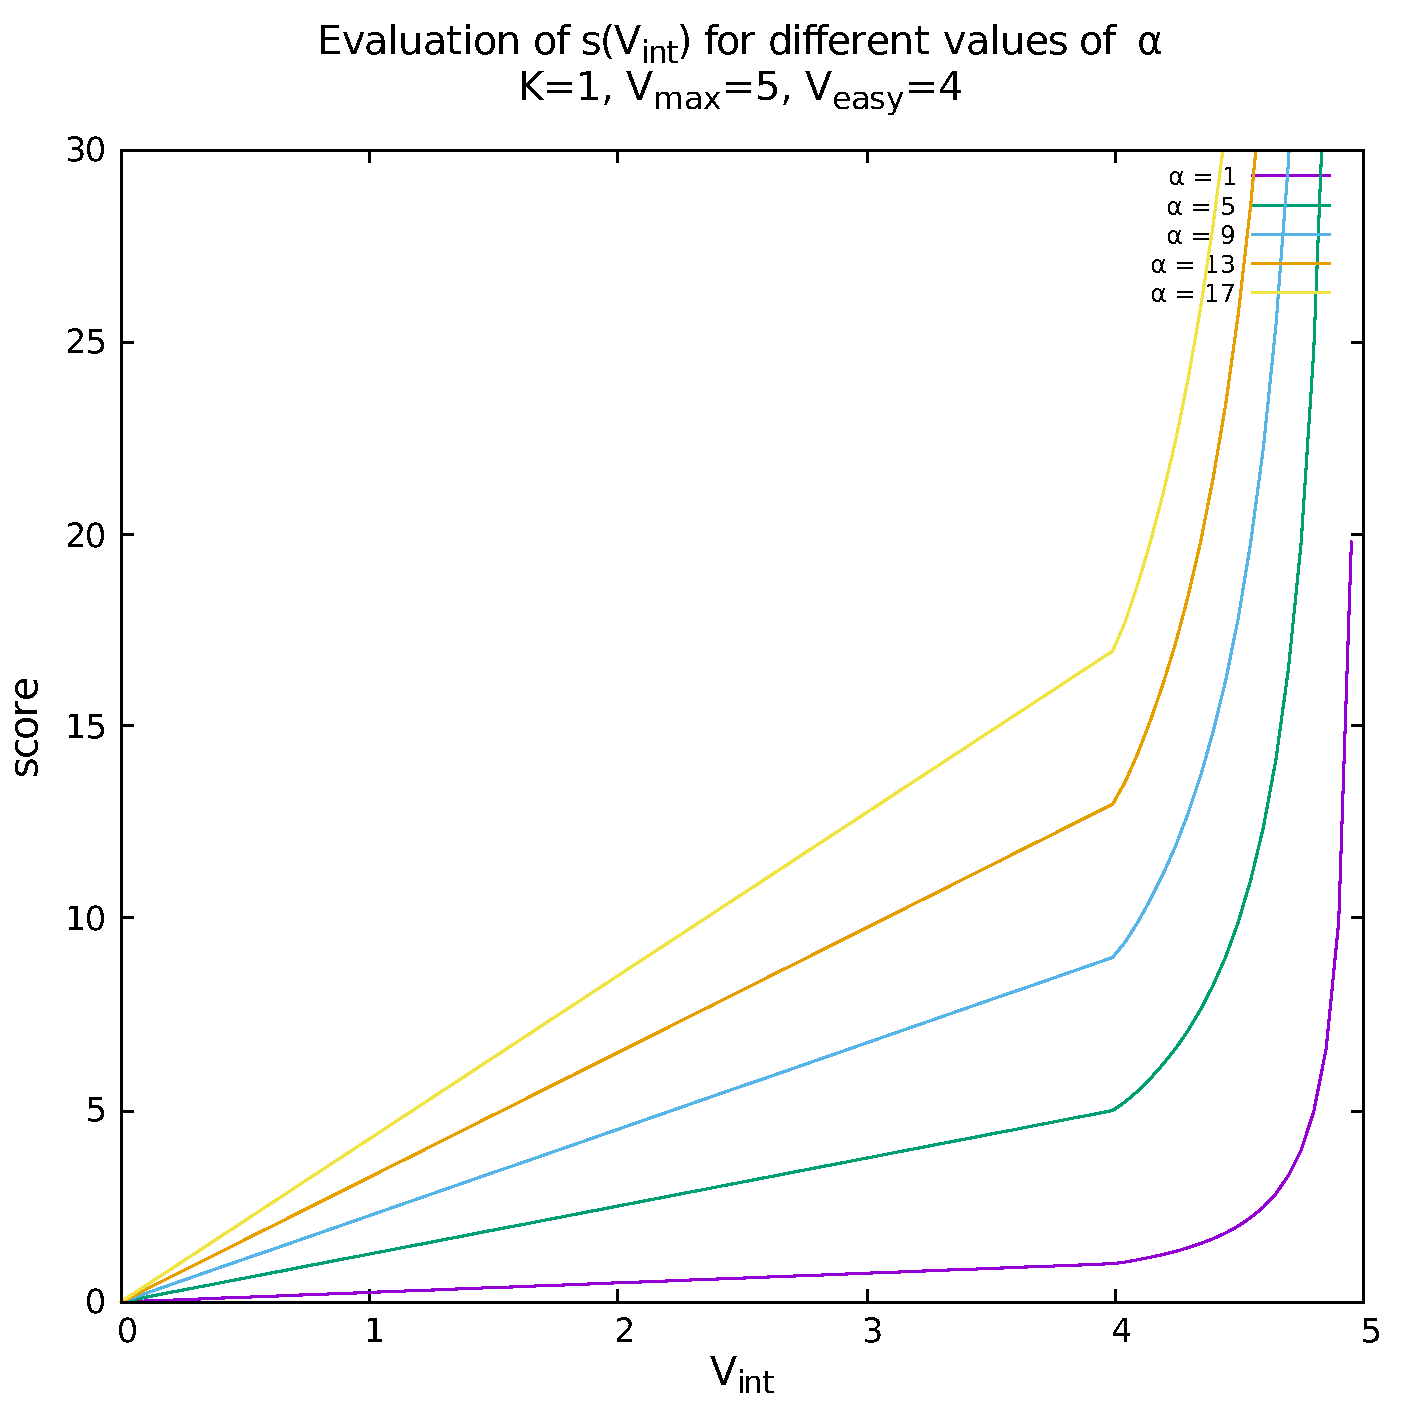
\includegraphics[height=3in]{./Graphics/score_alpha}
  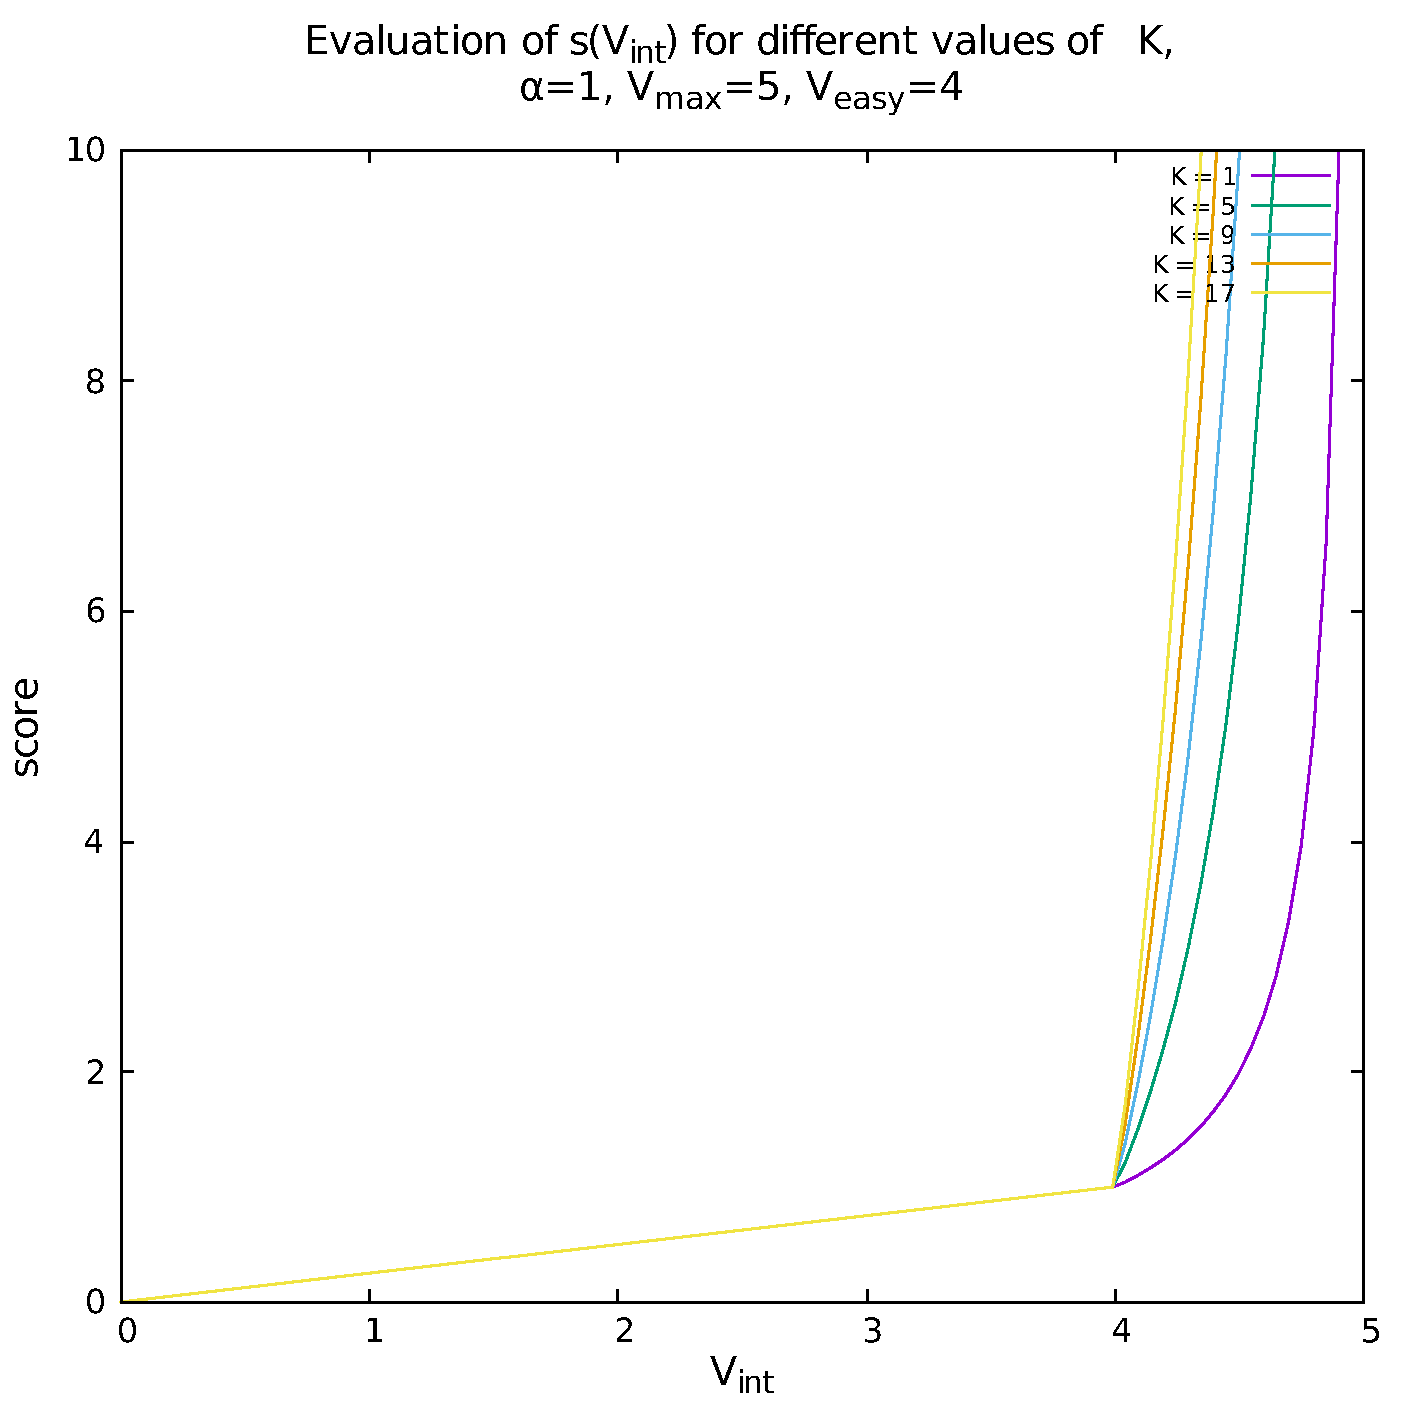
\includegraphics[height=3in]{./Graphics/score_k}
  \caption{Resulting score function for different values of $\alpha$ (top) and
  $K$ (bottom)}
\end{figure}

\subsection{Object representation as elementary shapes} \label{sec:shapes}
A good representation of objects is essential in order to compute efficiently
their intersection. In this project, objects have been represented by means of a
uniform data structure breaking down complex meshes to the union of simpler
shape, as done with the \emph{Constructive Solid Geometry (\emph{CSG})} tools of
most mainstream CAD application. Each object is represented, for the purpose of
grasp computation, by means of simpler, basic shapes, associated to their pose
relative to the object's reference system. These will be called
\emph{primitives}. A tree structure can also be created
by considering compound objects created in this manner to be a shape type on
their own, thus allowing recursive object building. This is similar to what the
\emph{assembly} and \emph{group} tools of mainstream CAD application do, as well
as what the library used for mesh representation (Assimp) does for
multiple-nodes meshes. This approach has a serie of advantages:
\begin{itemize}
  \item{Every object shares a common data structure. This makes it easier for
      the intersection algorithm to be as general as possible with little to no
    effort;}
  \item{the tree representation of the object makes it easy to save single or
      multiple objects to file and to create objects' configuration by-hand,
      which is useful both for debugging and for execution purposes (for
      example, the database of objects, together with their shapes, can be made
    distributed with no effort and version control tools can be useful);}
  \item{using an approach similar to what is supported by mainstream CAD
      applications results in the possibility of scripting the latter in order
      to automatically produce an exact representation of the object starting
      from a CAD model, which could be the same used for training in sec.
    \ref{sec:cad-mesh};}
  \item{the approach is very flexible because of the relative independency
      between the object's model and the rest of the algorithms: new use-case of
      the algorithm (e.g. for moving or nonrigid objects) could leave this part intact, and
      only work by modifying the informations about the position of the whole,
    or part of, the object.}
  \item{new, complex shapes which have to be implemented in future can be added
      to the primitive shapes as an extension, without the need of rebuilding
      the whole objects' database. This is the main advantage of using an
      object-oriented approach based on polimorphism for the implementation of this
    part.}
\end{itemize}

For this project, four main shape types have been implemented, and with these
the whole set of objects kept in consideration have been succesfully
represented.

Each primitive is represented by its shape type and a set of dimensions, which
is checked at runtime to be coherent to the associated shape. To the shape is
associated a pose information, represented as an affine transformation as in the
rest of the project. To each shape type functions have been implemented to
recognize whether a it intersects with, or contains, a point, an edge, a line, or
another shape. When computing intersections, these are efficiently used asZ c
special cases to recognize whether an intersection exists or not before
eventually running the computationally expensive intersection's volume
algorithm.

\paragraph{A \emph{cuboid}} is a shape representing a parallelepiped. It is represented by
three dimensions: its width $W$, its height $H$, and its depth $D$; its origin is fixed in one
of its corners, and its reference system's axis are on its edges' directions:
width extends over the $X$ axis, height extends over the $Y$ axis, and depth
extends over the $Z$ axis.

A point $P$ (in normalized homogeneous coordinates, i.e. with $w=1$  can be checked for belonging a cuboid $C$ of dimensions $(W,H,D)$ and
pose $A$ by first representing it into
the cuboid's coordinate system, and then checking its coordinates to be into the
cubes'dimensions:

\begin{equation}
P \in C \Leftrightarrow \begin{pmatrix}0\\0\\0\\1\end{pmatrix} \leq A^{-1}P \leq
\begin{pmatrix}W\\H\\D\\1\end{pmatrix}
\end{equation}
  
A line segment $L$ intersects the same cuboid if, by projecting it on one axis at a time,
all the three projections belong to the projection of the cube:

\begin{equation}
  L \in C \Leftrightarrow \left(L_x \in C_x\right) \wedge
  \left(L_y \in C_y\right) \wedge \left(L_z
    \in C_z\right)
\end{equation}

\paragraph{A \emph{sphere}} is a shape representing a sphere of fixed radius,
which is the only one of its dimensions. The reference system of the sphere, 
which its transformation refers to, is fixed into the sphere's center. Having
central simmetry, the rotation part of the sphere's transformation will actually
be ignored.

A point $P$ belongs to a sphere $S$ of radius $R$ if, after moving it into the
sphere's reference system, its distance from the origin is less then the radius:

\begin{equation}
  P \in S \Leftrightarrow \left(A^{-1}P\right)_{x,y,z}^2 < R^2
\end{equation}

Also, a line $L$ belongs to the same sphere if its distance from the origin is less
than $R$.

\paragraph{A \emph{cylinder}} is a shape representing a rect, circular cylinder.
Its two dimensional values represent the base's radius and the height of the
cylinder. Its coordinate system is fixed at the center of the circle, at the
base of the cylinder, with the
Z axis pointing upwards on the length direction.

A point $P$ belongs to a cylinder $C$ of radius $R$ and height $H$ if, after
moving it to the cylinder's reference system, its projection on the XY plane
belongs the base circle and its Z coordinate is lower than the cylinder's
height:

\begin{equation}
  P \in C \Leftrightarrow \left(A^{-1}P\right)_{x,y}^2 < R \wedge
  \left(A^{-1}P\right)_z > 0 \wedge \left(A^{-1}P\right)_z<H
\end{equation}

A line segment $L$ in the cylinder's reference system belongs to the same cylinder if its projection on the $XY$
plane belongs to the base circle and its projection over the $Z$ axis belongs to
the cilinder's height segment:

\begin{equation}
  L \in C \Leftrightarrow
  \left(L_{x,y} \in C_{x,y} \right)
  \wedge
  \left(L_{z} \in [0,H] \right)
\end{equation}

\paragraph{A \emph{compound}} is the composition of any number of shapes, called
\emph{children}. Children can be compounds too. This shape has no dimension
information, but only a reference system to which all the children's reference
systems are applied before any evaluation. For example, in order to transform a
point to a children's reference system for intersections' evaluation, the point
is first transformed using the compound's reference system, then it is
transformed again using the child's reference system. In this way, assembly-like
shapes can be formed.

A point, or any other primitive, $P$ belongs to a compound $C$ with children $c_i$ if it belongs to
\emph{at least} one of them:

\begin{equation}
  P \in C \Leftrightarrow \exists i : P \in c_i
\end{equation}

Using this four composing blocks, it is easy to form every object. Also, every
object can be evaluated for intersection with at least a point, which is the
base for the volumes' evaluation system described into sec.
\ref{sec:grasp_computing}; some objects can also be intersected more efficiently by
exploiting other special case features as line evaluation. Also, it has been
shown how the easy structure of each primitive, together with the use of
compounds, makes it easy to add further extensions to this system and immediately
make use of them.

\section{Efficient volume computation of objects' intersections} \label{sec:grasp_computing}
After defining the score function $d(V_{\text{int}})$, the only remaining
obstacle for computing the best possible grasping strategy is the actual
computation of shapes' intersections. 
